% \begin{frame}{Events grouped by longTracks vs DeltaR0 }
%     \begin{figure}
%         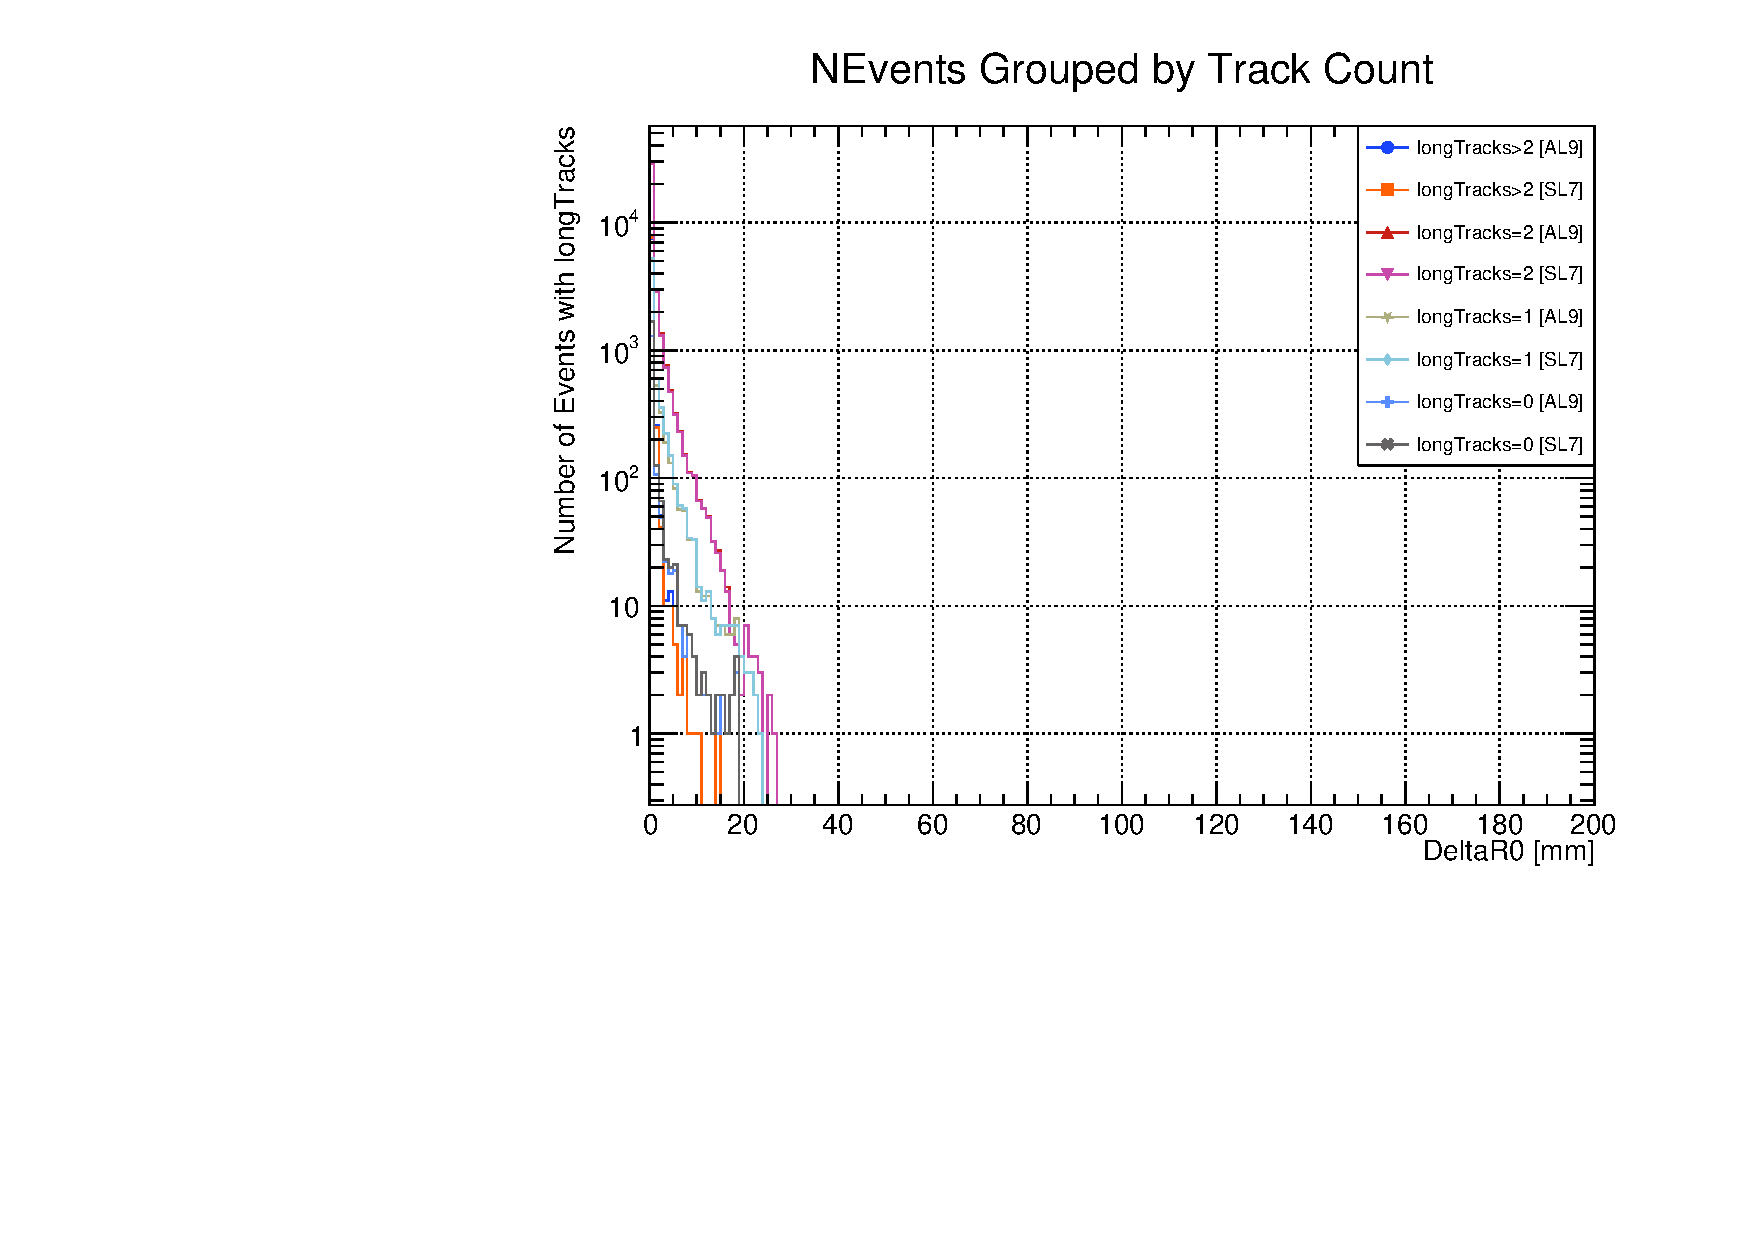
\includegraphics[width=\linewidth]{./output/DeltaR0_all.pdf}
%     \end{figure}
% \end{frame}

% \begin{subframe}{Events grouped by longTracks vs DeltaY0 [SKIP]}
%     \begin{figure}
%         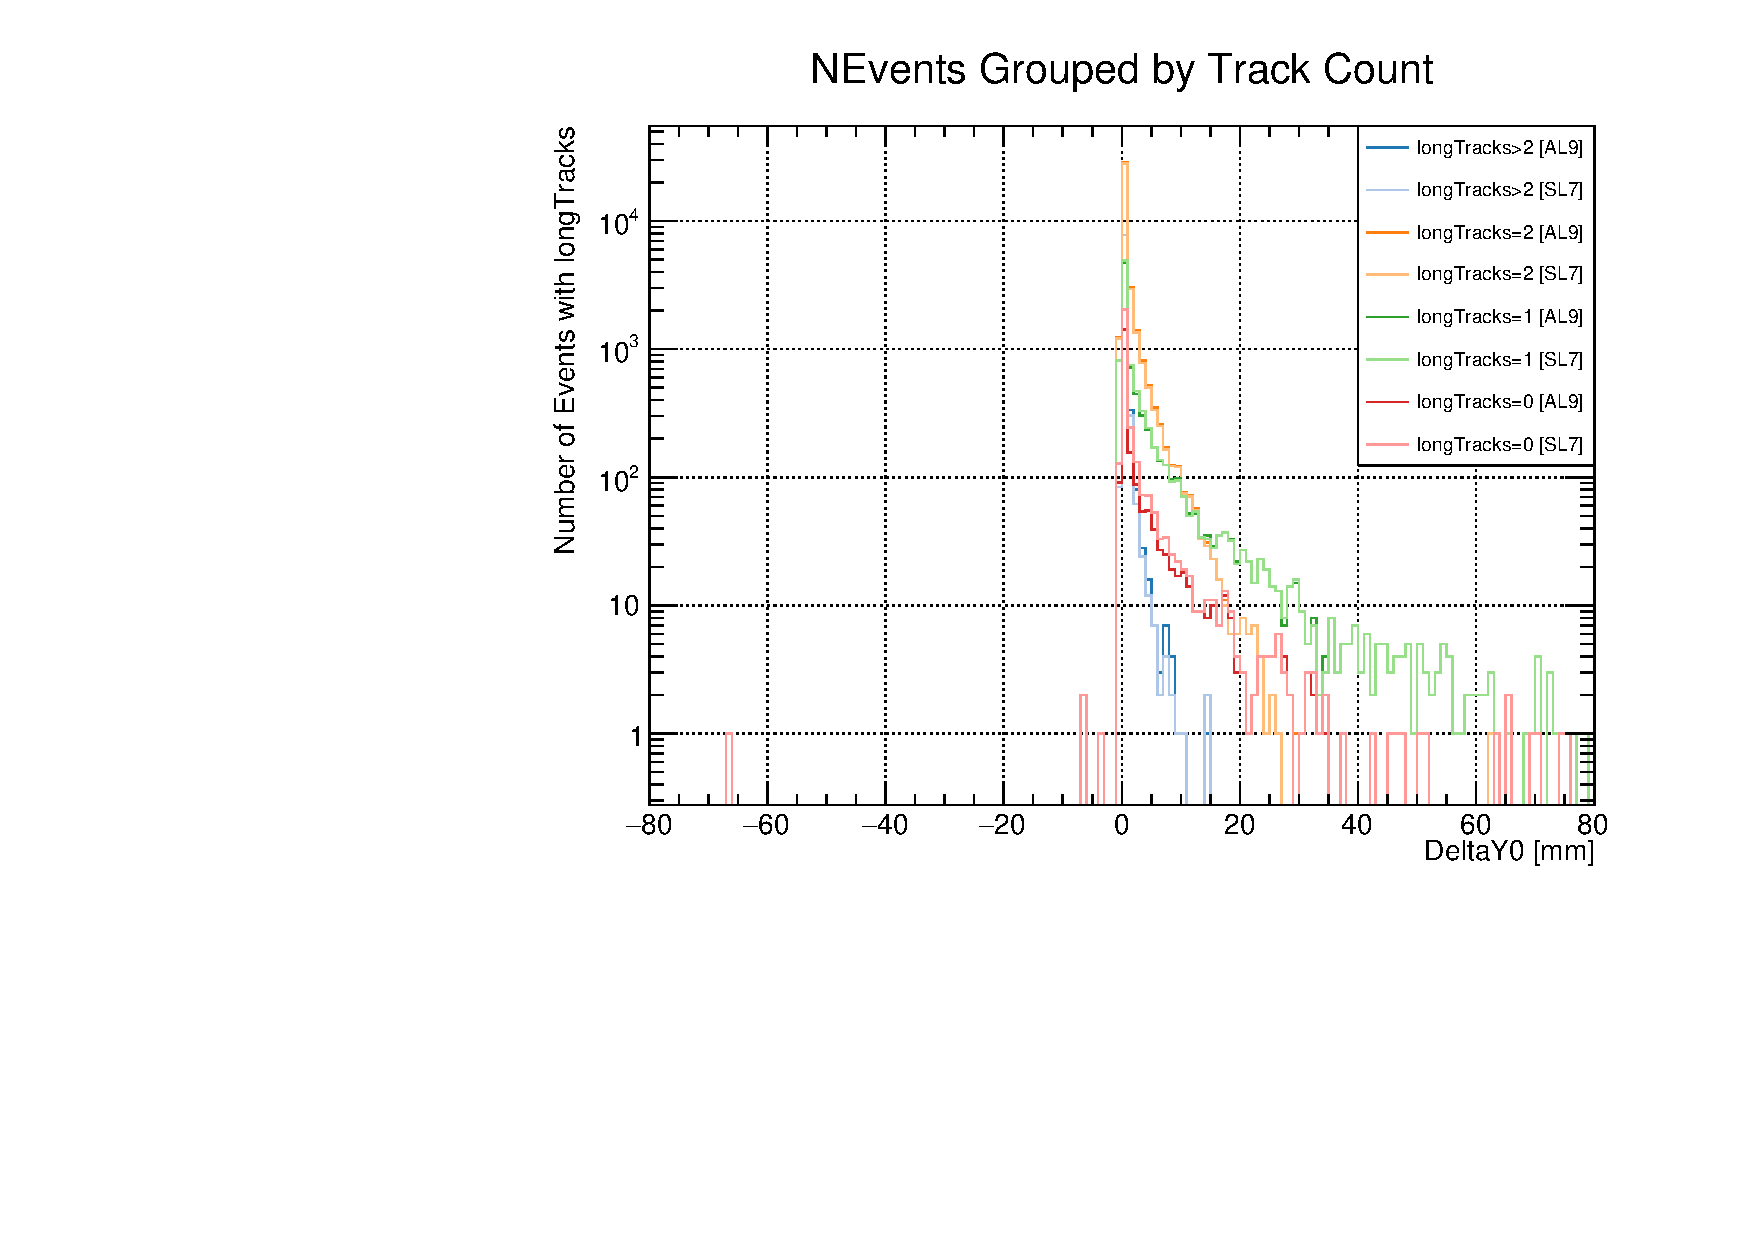
\includegraphics[width=\linewidth]{./output/DeltaY0_all.pdf}
%     \end{figure}
% \end{subframe}

% \begin{subframe}{Events grouped by longTracks vs DeltaX0 [SKIP]}
%     \begin{figure}
%         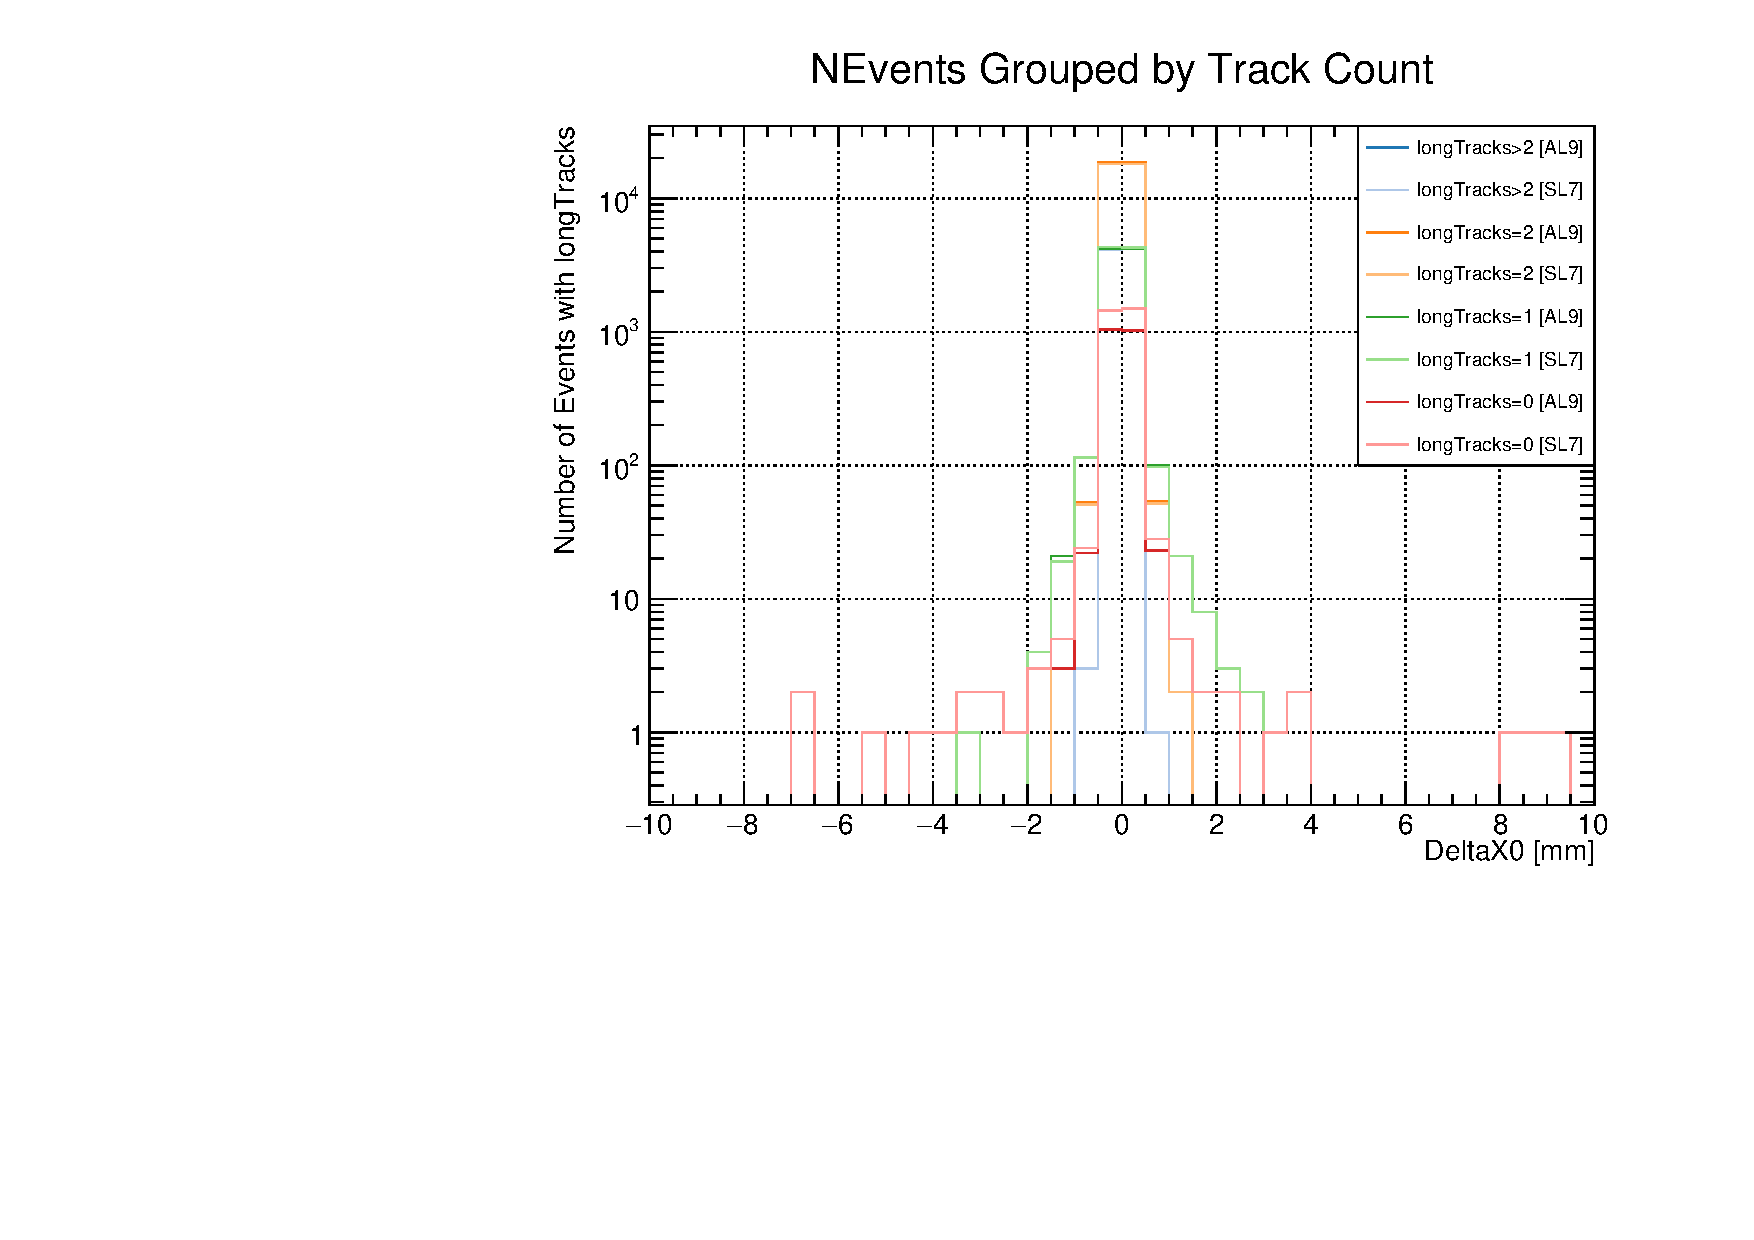
\includegraphics[width=\linewidth]{./output/DeltaX0_all.pdf}
%     \end{figure}
% \end{subframe}

% \begin{frame}{Events grouped by longTracks vs Theta0 }
%     \begin{figure}
%         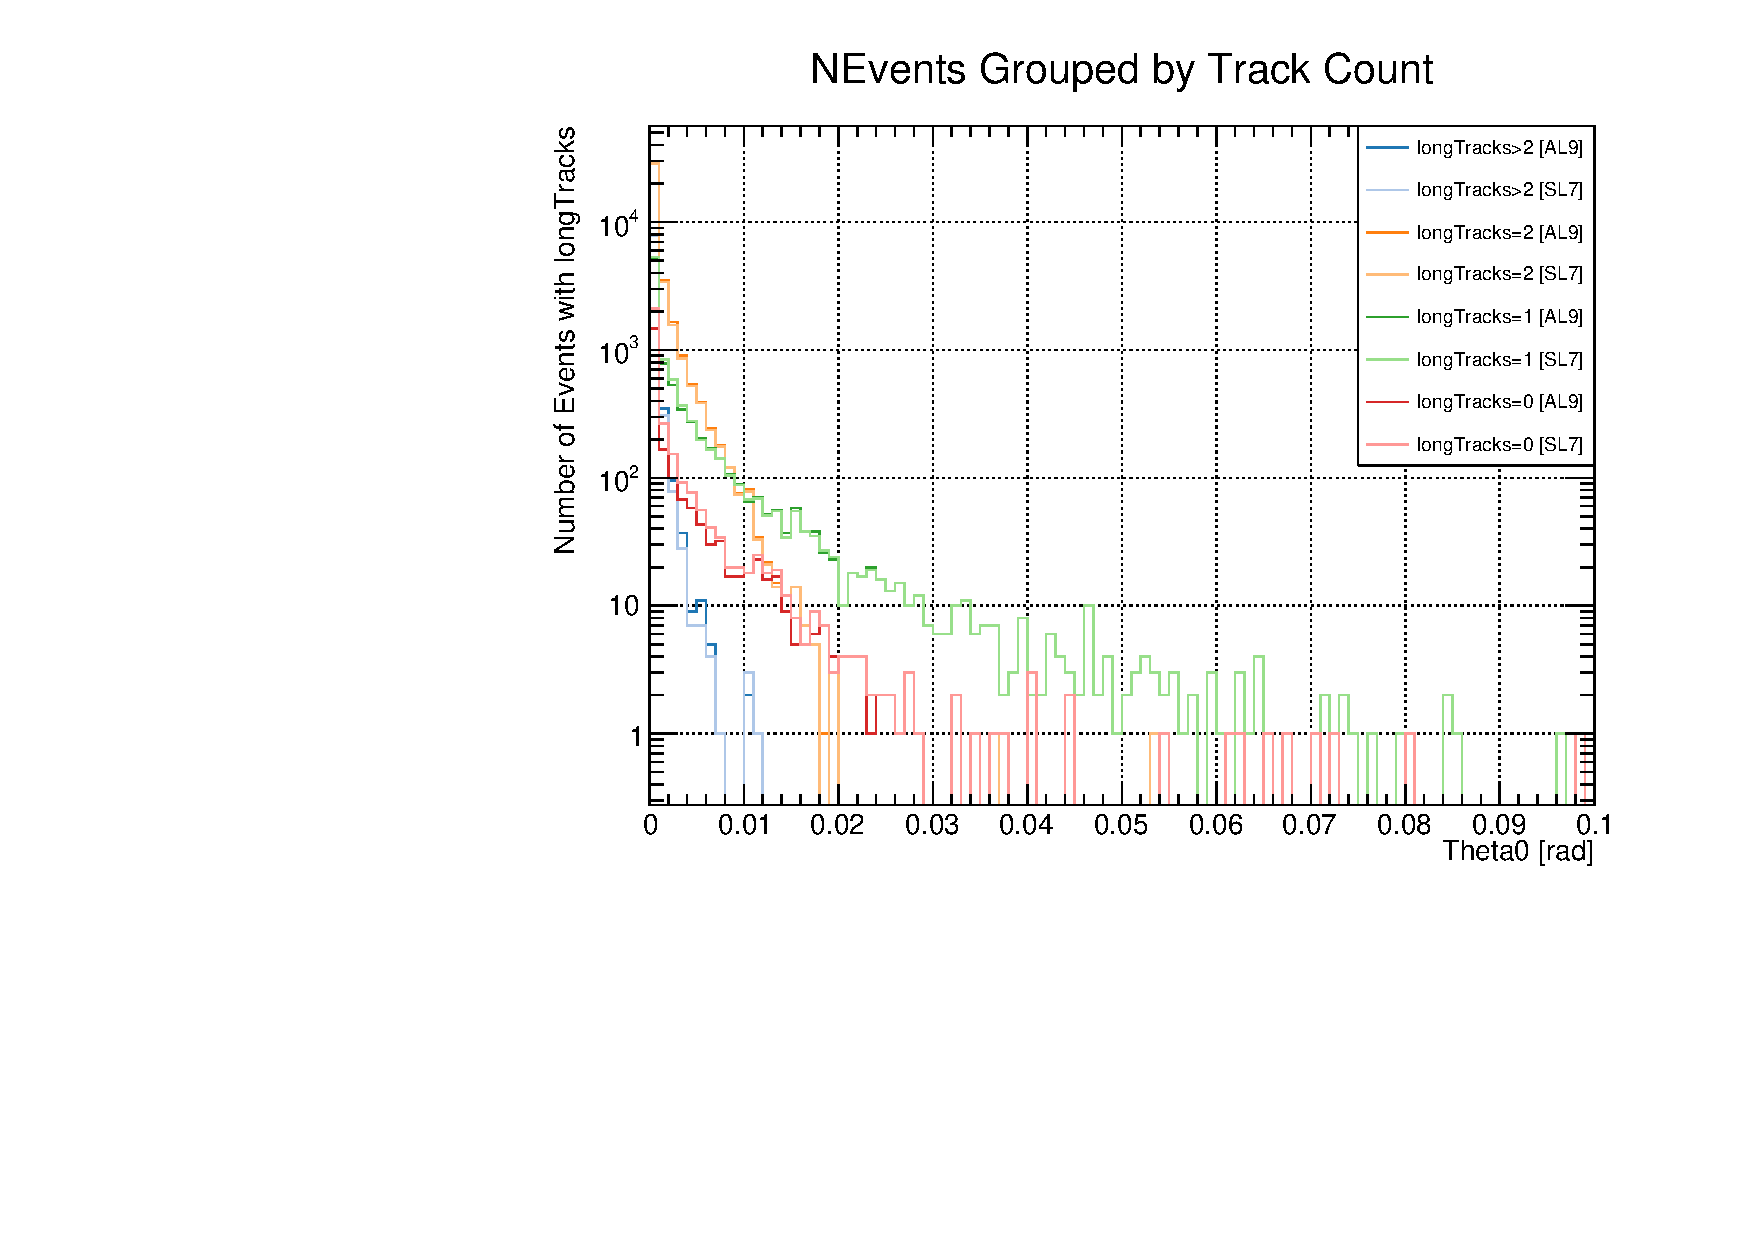
\includegraphics[width=\linewidth]{./output/Theta0_all.pdf}
%     \end{figure}
% \end{frame}

% % \begin{frame}{Two Track Reconstruction Efficiency }
% %     \begin{figure}
% %         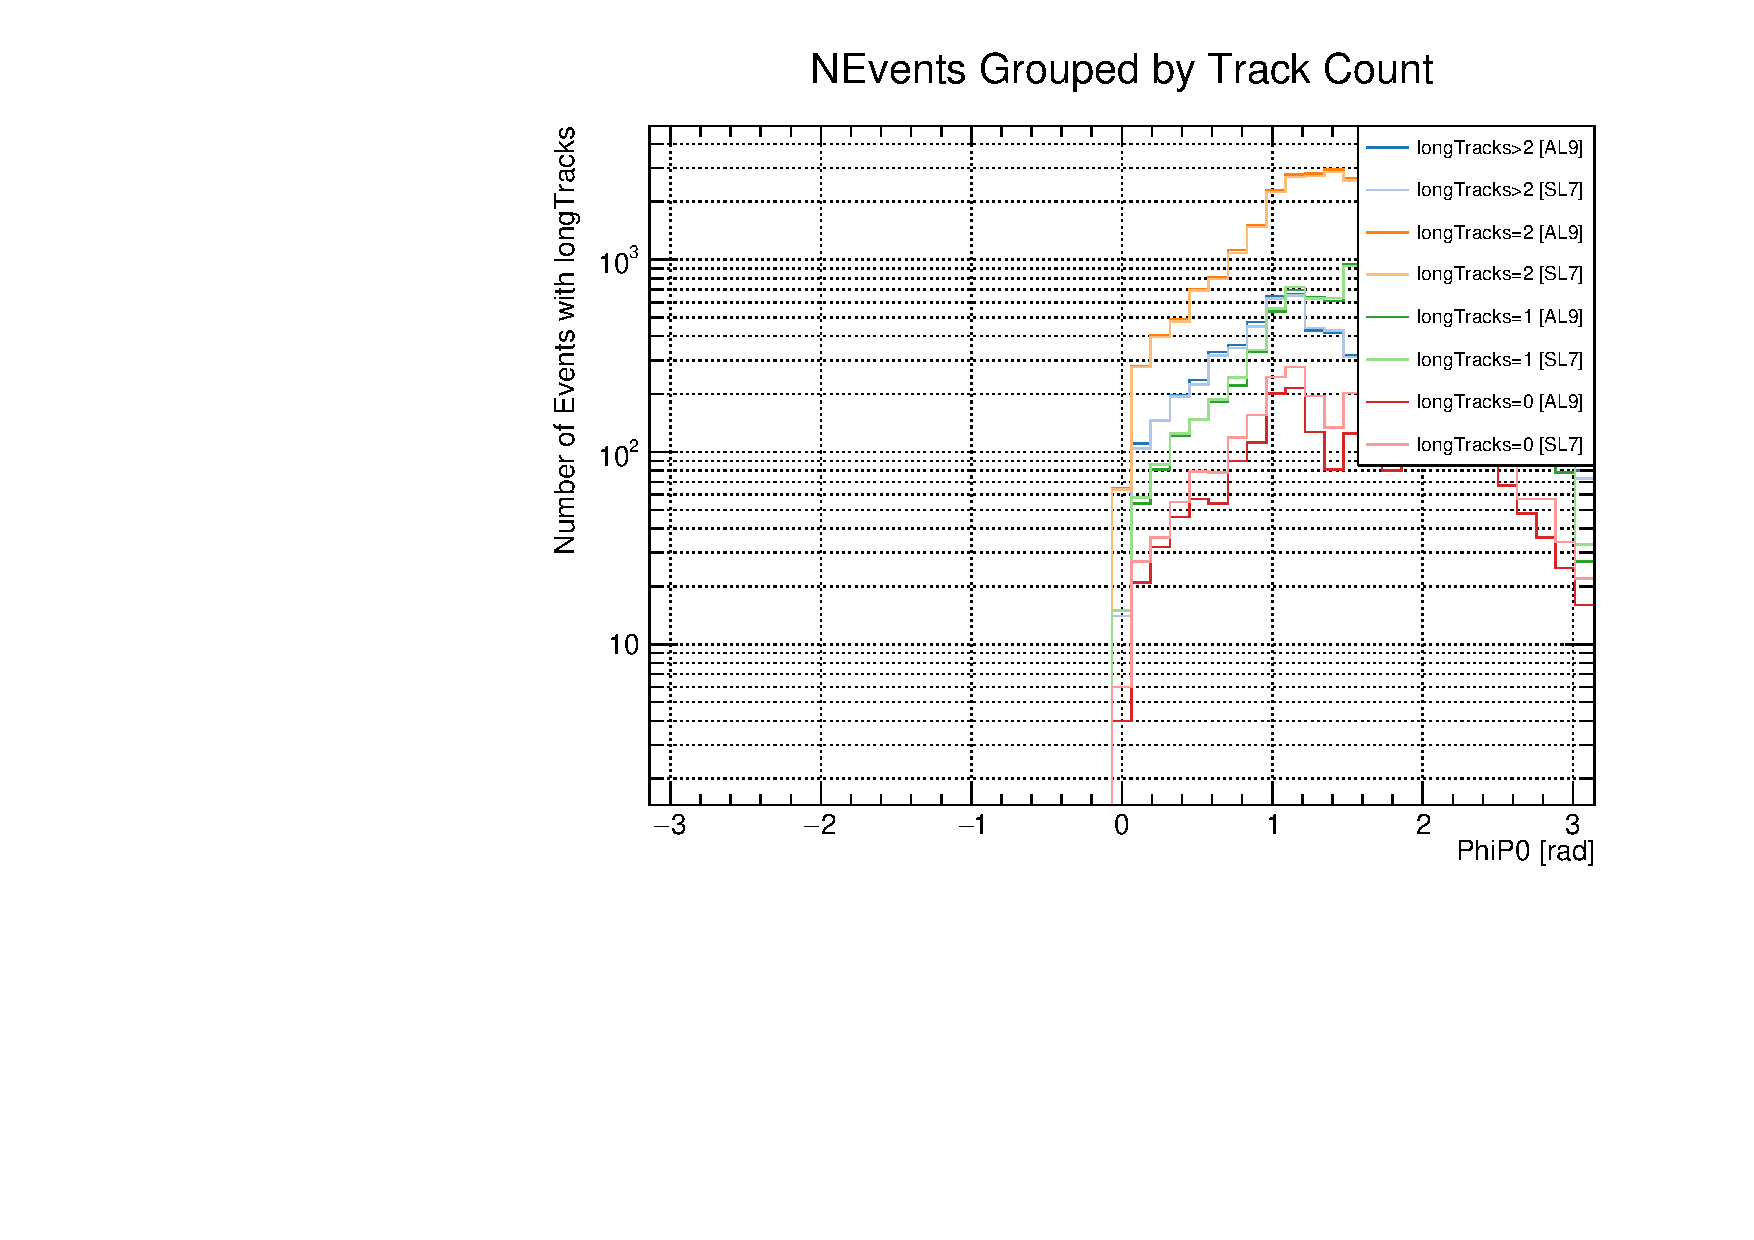
\includegraphics[width=\linewidth]{./output/Effi_PhiP0_all.pdf}
% %     \end{figure}
% % \end{frame}

% \begin{frame}{Events grouped by longTracks vs DeltaRP}
%     \begin{figure}
%         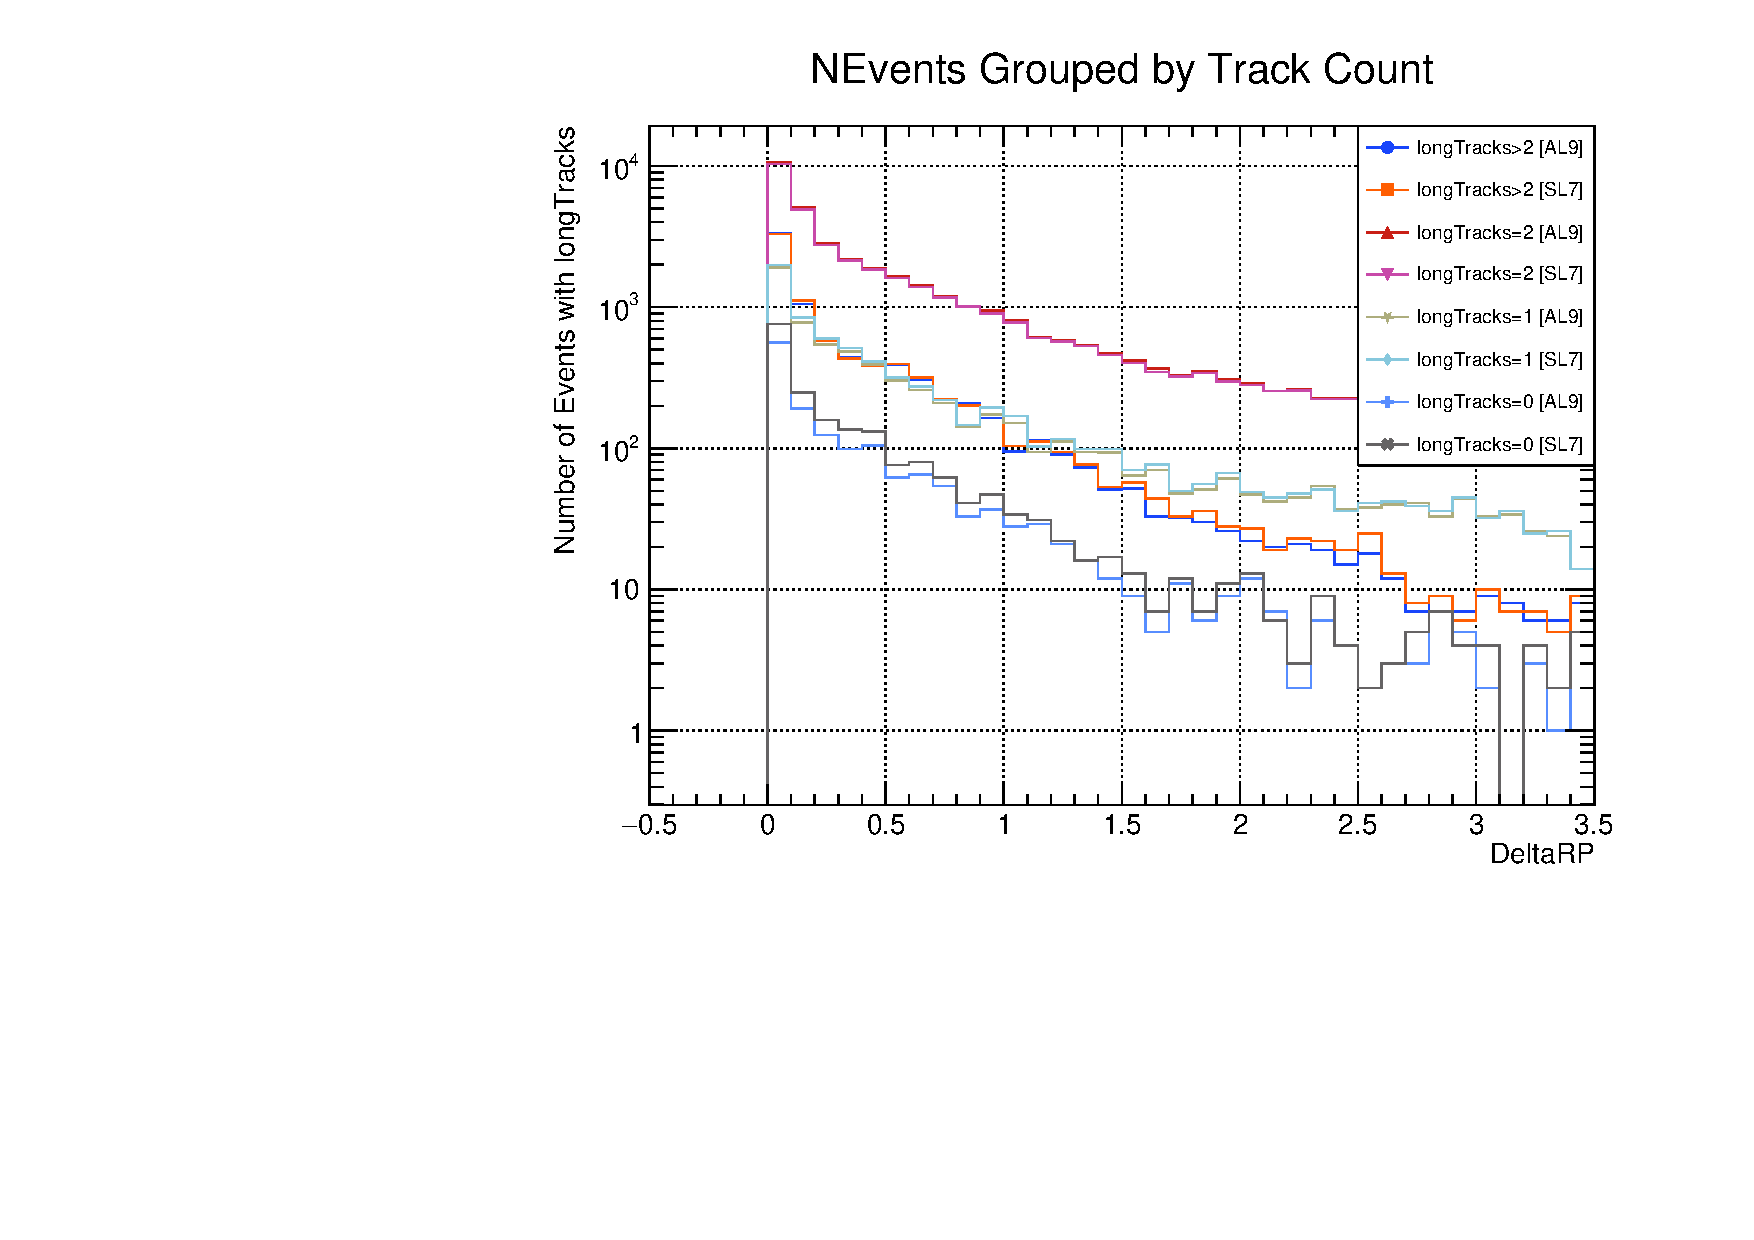
\includegraphics[width=\linewidth]{./output/DeltaRP_all.pdf}
%     \end{figure}
% \end{frame}

% \begin{frame}{Comments on longTrack grouped Plots}
%     \begin{itemize}
%         \item Good agreement between ALMA9 and CENTOS7
%         \item Events with $>2$ longTracks fall most rapidly [ 10 mm]
%         \item $=2$ longTracks decays less rapidly [nothing past 30 mm]
%         \item $=1, 0$ longTracks is relatively flat
%         \item {\color{red}Why do we reconstruct only one track at large separation?}
%     \end{itemize}
    
% \end{frame}